\documentclass[12pt]{article}

\usepackage{amsmath,amssymb,amsthm}
\usepackage{geometry}
\usepackage{enumerate}
\usepackage[shortlabels]{enumitem}
\usepackage{graphicx}

\usepackage{hyperref}

\begin{document}
\title{CS 6965 Advanced Data Visualization\\{\bf Project 3}}
\author{Yulong Liang (u1143816)}
\maketitle

\section*{Step 1: Dragon Demo (5 points)}

\begin{figure}[h]
\centering
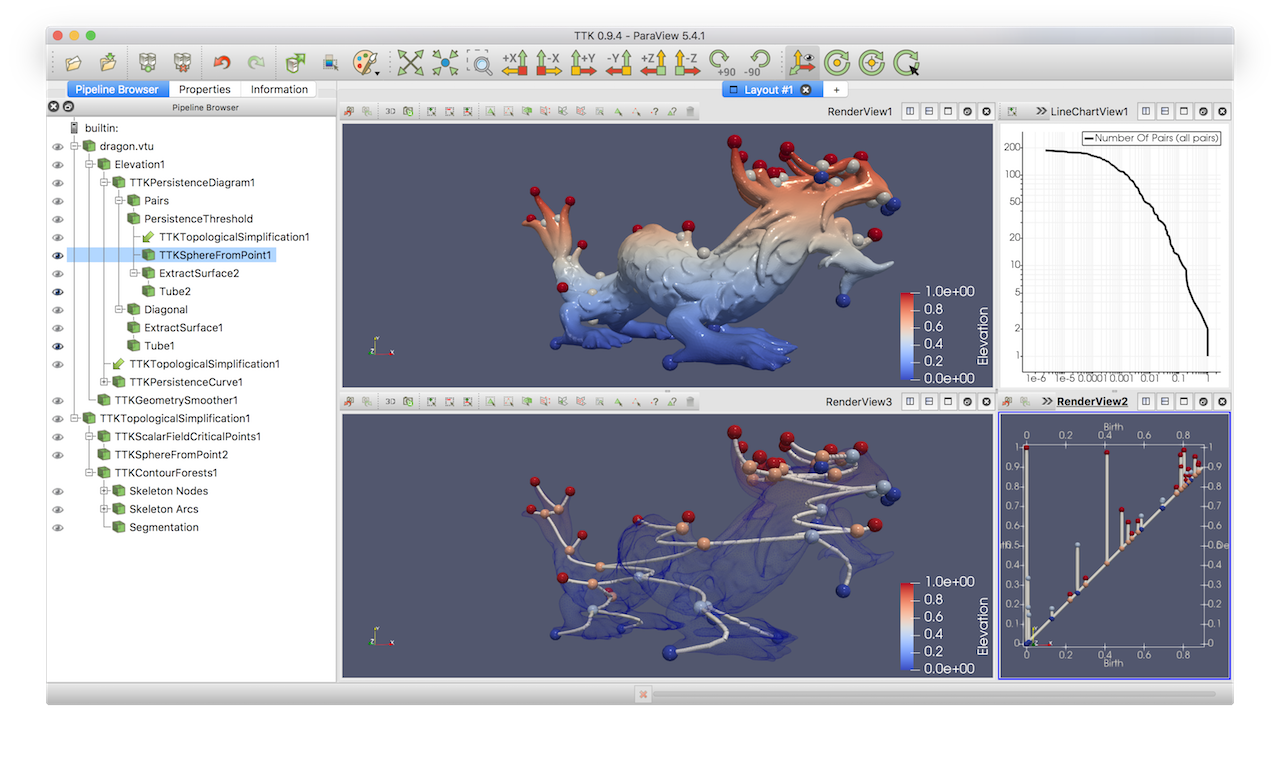
\includegraphics[width=1\linewidth]{2.png}
\caption{Screen capture of the Dragon Demo}
\label{fig:name}
\end{figure}

\newpage

\paragraph{Problem Encountered}
In the beginning, I strictly followed the instructions to make the contour tree. However, the colors of nodes in the Contour Tree are not identical to the colors of nodes in the Persistence Diagram even though they are both colored by \texttt{Nodetype}. Namely, the dark red points are displayed as light red in the contour tree.

\begin{figure}[h]
\centering
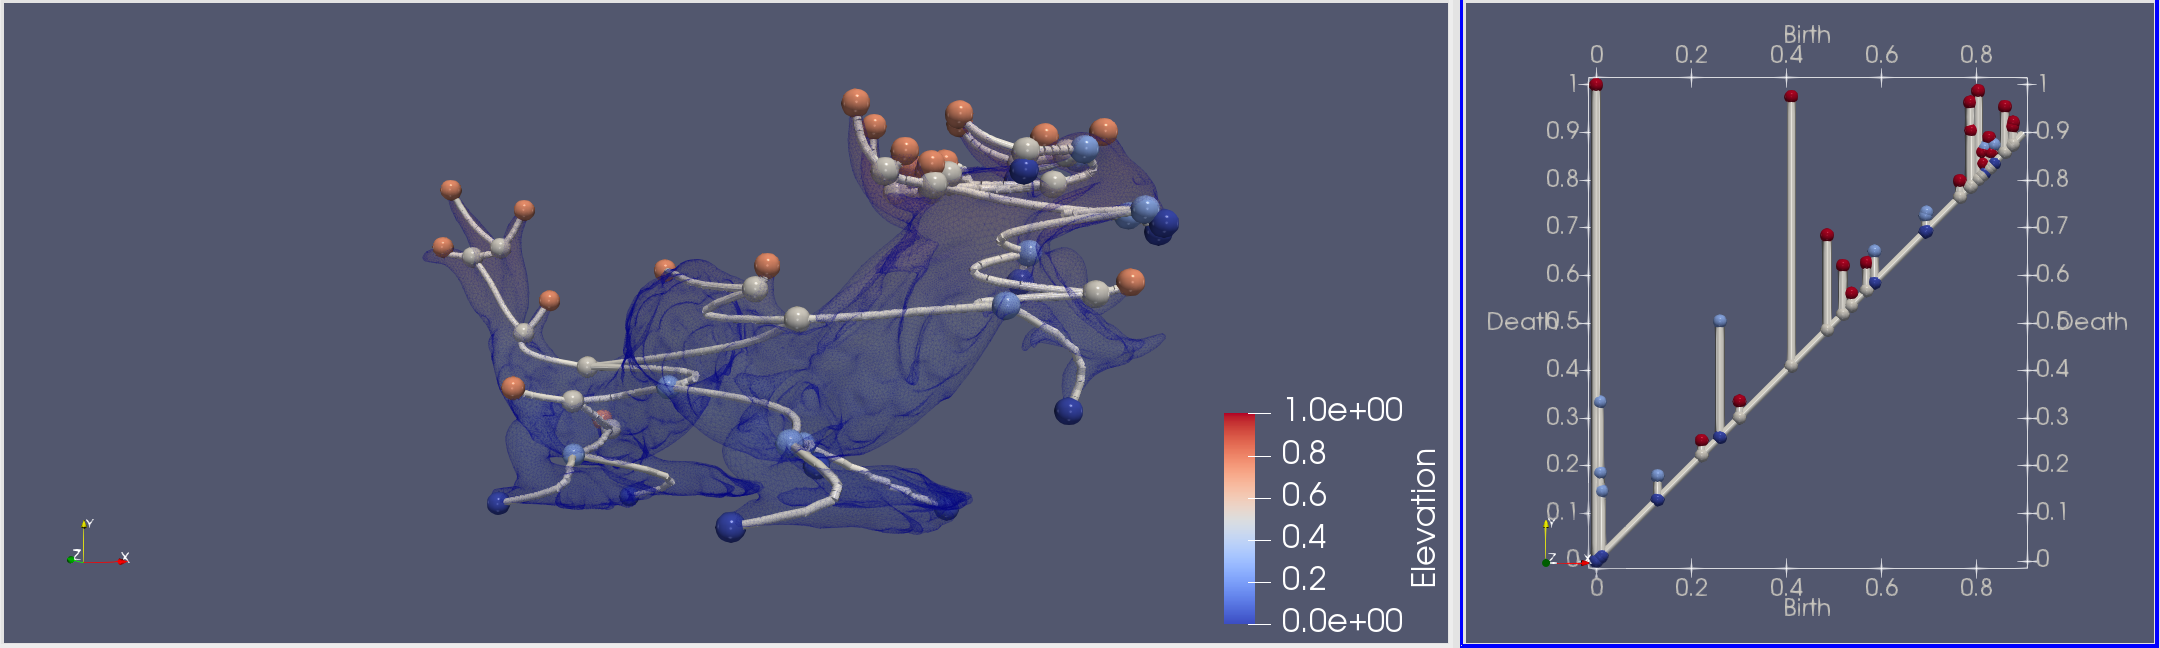
\includegraphics[width=0.5\linewidth]{2-1.png}
\caption{Problem on Contour Tree with blue-red color scale}
\label{fig:name}
\end{figure}

I also tried the same color as the demo, but still got a lighter green.
\begin{figure}[h]
\centering
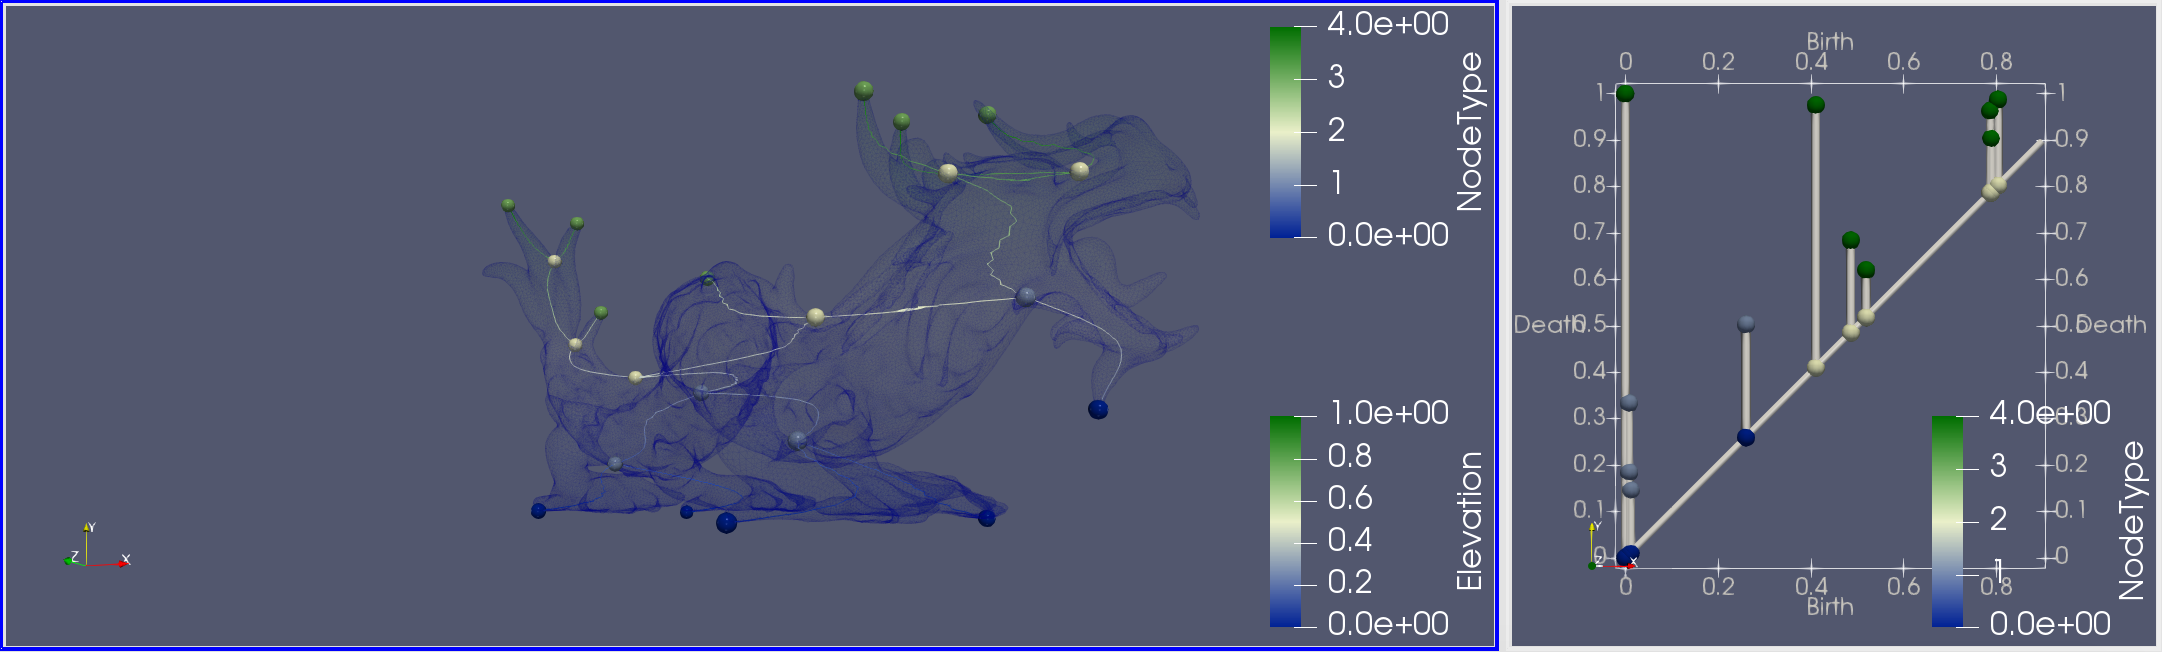
\includegraphics[width=0.5\linewidth]{2-2.png}
\caption{Problem on Contour Tree with blue-green color scale}
\label{fig:name}
\end{figure}

Finally I checked all the properties in the example state file and found that they used a difference color scale to enlarge the threshold of dark green.
\begin{figure}[h]
\centering
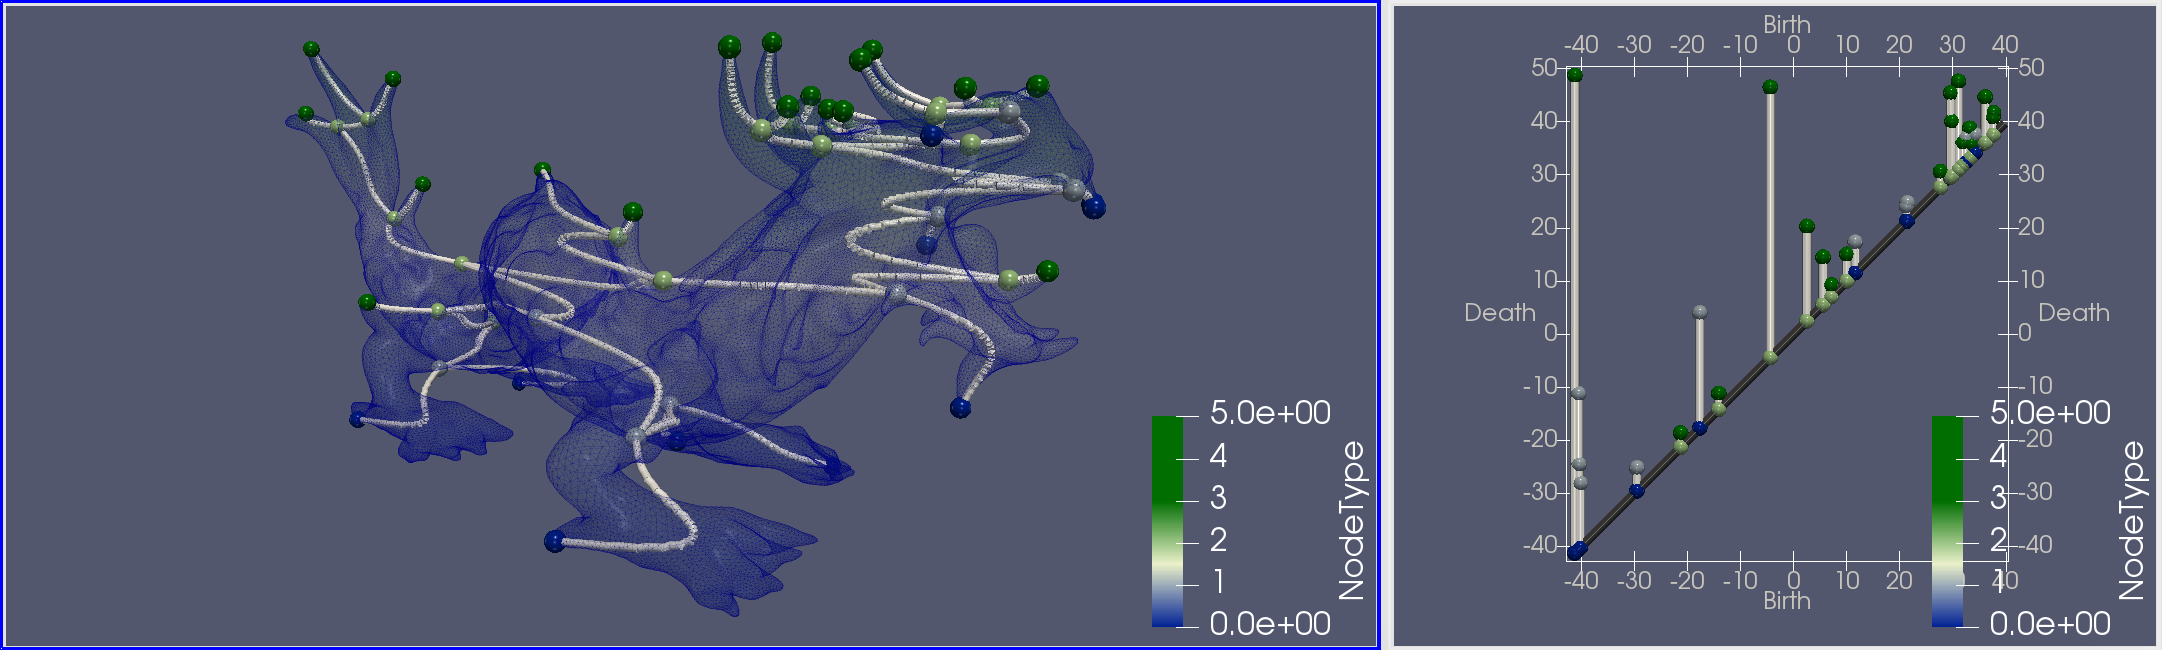
\includegraphics[width=0.5\linewidth]{2-3.png}
\caption{Color scale used in the example}
\label{fig:name}
\end{figure}

I accordingly modified my nodetype color scale and got a better look.

\end{document}